\documentclass[times, twoside]{zHenriquesLab-StyleBioRxiv}

\usepackage{newfloat}
\DeclareFloatingEnvironment[name={Supplementary Figure}]{suppfigure}
\DeclareFloatingEnvironment[name={Supplementary Table}]{supptable}
\usepackage{multirow}
\usepackage{makecell}
\usepackage{upgreek}

\newcommand{\ecoli}{\textit{E. coli}}
\newcommand{\dreca}{$\Delta$\textit{recA}} % ΔrecA
\newcommand{\teneighty}{RecB$_{1080}$} % RecB1080
\newcommand{\geneteneighty}{\textit{recB$_{1080}$}} % recB1080
\newcommand{\od}{OD$_{600}$} % OD600
\newcommand{\umsq}{$\upmu$m$^2$} % µm2
\newcommand{\ums}{$\upmu$m$^2$.s$^{-1}$} % µm2.s-1
\newcommand{\ncells}[1]{N$_{\text{cells}}$ = #1} % N_cells = {}
\newcommand{\nspots}[1]{N$_{\text{spots}}$ = #1} % N_spots = {}
\newcommand{\nnucl}[1]{N$_{\text{nucleoids}}$ = #1} % N_nucleoids = {}

% Surname of the lead author for the running footer
\leadauthor{Thédié} 

\begin{document}

\title{RecBCD binding time to DNA \emph{in-vivo} is an intrinsic property of the complex}
\shorttitle{RecBCD binding time to DNA \emph{in-vivo} is an intrinsic property of the complex}

\author[1]{Daniel Thédié}
\author[2]{Alessia Lepore}
\author[1]{Lorna McLaren}
\author[1,3]{Meriem El Karoui}


\affil[1]{Institute of Cell Biology, University of Edinburgh, Edinburgh, UK}
\affil[2]{Ecole Polytechnique, Paris-Saclay, France}
\affil[3]{Ecole Normale Supérieure, Paris-Saclay, France}  % ENS Saclay, to be checked by Meriem

\maketitle

\begin{abstract}
% Scene setting
Repairing DNA damage is of primary importance for living organisms. Double-strand breaks are one of the most serious types of DNA damage. In \ecoli, they are recognised and processed by the RecBCD complex, which initiates repair by homologous recombination.
% What is our main question?
While repair dynamics downstream of RecBCD have been well characterised, it is still unclear how long the complex stays bound to DNA, and what triggers its dissociation \emph{in-vivo}.
% What experimental setup did we use?
% What data did we produce?
To answer these questions, we imaged RecB at the single-molecule level, and recorded its response to different levels of DNA damage induced by the antibiotic ciprofloxacin.
% What is the main finding?
We found that dissociation of RecBCD from DNA is an intrinsic property of the complex, and does not depend on the amount of DNA damage, or on the next step in the repair pathway.
% General sentence on what the article contributes


\end{abstract}

\begin{keywords}
    DNA repair | RecBCD | Imaging | \emph{in-vivo}
\end{keywords}

\begin{corrauthor}
    meriem.elkaroui\at ed.ac.uk
\end{corrauthor}

\section*{Introduction}

% Endogenous DSBs
DNA double-strand breaks (DSBs) pose a serious threat to the integrity of bacterial cells. In \emph{E. coli}, a common source of DSBs is the collisions of the replication fork with DNA-bound proteins, which has been reported to occur in $\sim$18\% of cells per cell cycle\cite{Sinha2018} and leads to the disassembly of the replisome\cite{Michel1997}. The resulting Y-shaped DNA structure is bound by the RuvAB complex, which pulls the DNA strands (in a process called "branch migration") to create a "chicken-foot" four-way DNA structure\cite{Seigneur1998}. The free end of this structure (DNA tail) is bound by RecBCD, which either (i) digests the whole DNA tail and displaces RuvAB, allowing the replisome to be re-loaded, or (ii) recognises a Chi-site and loads the RecA protein onto the 3' end of the DNA tail\cite{Michel2001}. Since this part of the DNA was recently replicated, a homologous sequence is likely to be present in close proximity, and can be used for homologous recombination.

% Exogenous DSBs (ciprofloxacin)
\emph{E. coli} cells might also experience DSBs from exo\-genous sources, such as anti\-biotics. Ciprofloxacin is an antibiotic of the fluoro\-quinolones family, which causes DSBs. Im \emph{E. coli}, it does so by binding covalently to DNA topoisomerase II (gyrase), and trapping it in a DNA-bound conformation\cite{Kohanski2010}. The exact mechanism through which the DSBs are created is still unclear. Since the poisoned gyrase is tightly bound to DNA, it is likely to cause replication fork collisions\cite{Wentzell2000, Drlica2008}, and the subsequent repair of a chicken foot structure. Furthermore, the ciprofloxacin-poisoned gyrase is trapped in the "open" stage of its catalytic cycle, where it holds together two disjointed DNA ends. Therefore, upon removal of the gyrase (through a process that involves the ExoVII nuclease\cite{Huang2021}), we can reasonably expect the formation of a DSB independently of DNA replication\cite{Zhao2006}. Taken together, these studies suggest that in fast-growing cells, which contain multiple replication forks, both replication-dependent and independent DSBs occur.

% How DSBs get repaired
% RecBCD biochemistry (incl. dissociation from DNA)
In \emph{E. coli}, DSBs are repaired through the RecBCD pathway. RecBCD is a heterotrimeric protein complex, which combines several enzymatic activities\cite{Dillingham2008}. Upon recognition of a DSB, RecBCD translocates along the DNA at a speed of $\sim$1.6 kb/s, thanks to its combined 5' and 3' helicase activities\cite{Wiktor2018}. While translocating, RecBCD digests both DNA strands until it meets a specific 8-base pair sequence (5'-GCTGGTGG-3') called Chi-site. Upon recognition of the Chi-site, RecBCD pauses briefly before resuming translocation, albeit with modified nuclease activity: the 5' DNA end is be degraded more slowly, and the 3' end is not degraded at all, leading to a 3' DNA overhang. Of note, Chi recognition by RecBCD is not systematic, and was previously reported to occur with $\sim$40\% probability by an \emph{in-vitro studies}\cite{Taylor1992}. As RecBCD creates the 3' overhang, the nuclease domain of its RecB subunit promotes loading of the RecA protein onto the single-stranded DNA (ssDNA)\cite{Churchill2000, Spies2006}. The resulting RecA-DNA nucleoprotein filament is used as a template to search for an intact homologous sequence and perform homologous recombination. It is still unclear at which point exactly RecBCD dissociates from the DNA and what specificly triggers the dissociation. One \emph{in-vitro} study suggested that RecBCD dissociation was triggered by Chi recognition\cite{Taylor1999}, but the RecA filament could also play a role.

% General response to DNA damage (SOS and nucleoid compaction)
DSB repair is the first step of a general response to DNA damage known as the SOS response\cite{Baharoglu2014}. The formation of the RecA nucleoprotein filament triggers the auto-proteolysis of the LexA transcriptional repressor, which results in the activation of the genes of the SOS regulon. Among those are RecA, inhibitors of cell division such as SulA, and the SMC (structural maintenance of chromosomes)-like protein RecN. As a result, the cells elongate\cite{Bos2015}, and their DNA is compacted at the cell centre\cite{Odsbu2014}. This response facilitates homologous recombination between sister chromosomes, and ensures that cell division does not take place before paired chromosomes have been correctly separated.

% RecB/RecA mutants
Mutants in the repair pathway are affected in their ability to repair DSBs. Cells that are \emph{recA}-deficient (\dreca) are entirely unable to repair DSBs through homologous recombination, and the prolonged action of RecBCD on the DNA results in the digestion of large parts of the chromosome\cite{Horii1968, Chow2007}. \emph{recA}-deficient cells are however capable of repairing DSBs arising from fork reversal, thanks to RecBCD's exonuclease activity\cite{Seigneur1998, Michel2001}. The $D_{1080} \rightarrow A$ point mutation in the RecB subunit of the RecBCD complex (\teneighty) abolishes RecB's nuclease activity, as well as its ability to load the RecA protein on DNA\cite{Yu1998, Wang2000}. The other activities of the complex (DSB recognition, DNA unwinding, Chi-recognition) are unaffected\cite{Anderson1999}. Despite the loss of its RecA loading activity, the \teneighty\ mutant is still able to repair DSBs. \teneighty CD unwinds DNA at the break without degrading it, and the Single-Strand Binding protein (SSB) coats the 3' ssDNA, while the RecJ exonuclease degrades the 5' ssDNA. Finally, the RecFOR complex displaces SSB and load RecA, allowing for homologous recombination to occur\cite{Ivancic-Bace_2003}.

% Previous microscopy studies of DSB repair
Previous microscopy studies have shed light on different aspects of DSB repair by RecBCD. Several \emph{in-vitro} studies have quantified the rate of DNA unwinding by RecBCD\cite{Spies2003,Liu2013}, as well as the growth rate of RecA filaments\cite{Joo2006,Galletto2006,Handa2009} and the mechanism of homology searching\cite{Forget2012,Ragunathan2012}. These studies imaged single DNA strands during unwinding or RecA filament formation, sometimes with the help of Förster Resonance Energy Transfer (FRET)\cite{Joo2006,Ragunathan2012}. Complimentary to the \emph{in-vitro} work, \emph{in-vivo} studies have provided more insight into DNA end resection by RecBCD\cite{Wiktor2018}, confirming the complexe's translocation speed and high processivity. More recently, the diffusion of RecB was quantified \emph{in-vivo} at the single-molecule level\cite{Lepore2023}. The spatial organisation of RecA during DSB repair has been extensively characterised. Studies reported the presence of RecA foci\cite{Renzette2005,Renzette2007,Centore2007,Amarh2018}, filaments\cite{Kidane2005}, or bundles of filaments\cite{Lesterlin2013,Ghodke2019}. The homology search and pairing processes were also observed \emph{in-vivo}, showing that DSBs are brought to the centre of the cell during the repair process\cite{Badrinarayanan2015,Wiktor2021}. Of note, RecA imaging is particularly challenging because fluorescent protein fusions are not functional (or only partially). To circumvent this problem, previous studies have used partially functional fusions to fluorescent proteins\cite{Kidane2005,Renzette2005,Renzette2007,Centore2007,Lesterlin2013,Klimova2020}, tandem fusions where the fluorescent fusion is expressed alongside the wild-type protein\cite{Amarh2018,Wiktor2021}, fluorescent fusions to a phage protein that specifically binds RecA filaments\cite{Ghodke2019} or a fusion to the ALFA tag\cite{Wiktor2021}.

% Overview of the article
In this study, we aimed to learn more about the repair of ciprofloxacin-induced DSBs by RecBCD and RecA. We took advantage of RecBCD's low copy number ($\sim$5 molecules per cell on average\cite{Lepore2019a}) to perform enhanced localisation microscopy\cite{Yu2006, Elf2007} using a fully functional fusion of RecB to the Halo-tag that was previously developed and tested in the lab\cite{Lepore2019a}. This allowed us to detect and localise DNA-bound RecB molecules \emph{in-vivo}, and to estimate how long RecBCD stays bound to DNA. By exposing cells to different ciprofloxacin concentrations during imaging, we were able to look at the evolution of the repair process over time, and assess how cells were coping with different levels of DNA damage. To broaden our view of the repair process, we imaged a fluorescent fusion to the RecA protein in the same conditions, using a tandem fusion of RecA to the SYFP2 fluorescent protein that was previously shown not to affect its function\cite{Wiktor2021}. Finally, imaging RecB in the \dreca\ and \teneighty\ mutants gave us insight into the factors that might affect RecBCD's dissociation from the DNA.


\section*{Materials and Methods}

\subsection*{Strain construction}
\textit{E. coli} MG1655 and derivatives were used in this study. A list of all strains and plasmids used are presented in Supp. Tables \ref{SItab:strains} and \ref{SItab:plasmids}.
MEK2623 (RecB-Halo RecA-SYFP2) was constructed by transferring the RecA-SYFP2 tandem fusion by P1 transduction, using EL2514\cite{Wiktor2021} as a donor and MEK65\cite{Lepore2019a} as a receiver. The clones were selected on Kanamycin plates, and checked by Sanger sequencing. MEK2622 (\dreca) was constructed by tranferring the \textit{recA} deletion by P1 transduction, using BHC9 as a donor, and MEK65 as a receiver. MEK2629 was obtained by transforming the pDT6 plasmid (gift from Mark Dillingham) into the MEK65 strain by heat-shock.

\subsection*{Microscopy samples preparation}
For all experiments, the cells were grown in M9 supplemented with 0.2\% (w/v) glucose, 2 mM MgSO$_4$, 0.1 mM CaCl$_2$, 1X MEM Essential and MEM non-essential amino acids (Gibco).
\subsubsection*{Cell culture}
Cells were grown overnight from a -80\celsius\ glycerol stock in 5 mL medium at 37\celsius, shaking at 150 rpm. In the morning, the cells were diluted 1:300 into 15 mL of medium and grown at 37\celsius, shaking at 150 rpm until they reached an \od\ of 0.2-0.3 (mid-exponential phase).
Alternatively, a 15 mL culture was inoculated using a -80\celsius\ glycerol stock, and placed at 37\celsius\ with stirring in a turbidostat device (OGIBio), which measured \od\ and diluted cells at 3 min intervals, in order to keep them at a constant \od\ of 0.2.
\subsubsection*{Halo labelling}
The same labelling protocol as in \cite{Lepore2023} was used. A volume of cells equivalent to 1 mL at \od=0.2 was centrifuged (8000 rpm) and resuspended in 1 mL of fresh medium. 5 µL of JF549 dye (Janelia Fluor Halo-tag Ligand, Promega) was added (final concentration 1 µM) and the cells were further incubated for 1h at 37\celsius\ in the dark, shaking at 150 rpm.
\subsubsection*{DNA labelling}
When relevant, cellular DNA was labelled by adding Sytox Green (Invitrogen) at a concentration of 500 nM, at the same time as the JF549 dye. It was incubated as described above.
\subsubsection*{Gam overexpression}
For experiments where Gam was over-expressed, arabinose was added to the cells during the labelling step, at 1\% final concentration. Arabinose (at the same concentration) was also added to the medium for subsequent washes, and in the agar-pad to maintain exposure during imaging.
\subsubsection*{Dye removal}
The cells were centrifuged for 3 min at 8000 rpm, the supernatant discarded, and the pellet resuspended in 1 mL of fresh medium and transferred to a new tube to avoid the dyes sticking to the plastic of the tube. This procedure was repeated 3 times to fully remove unbound dye. The cells were finally resuspended in 200 µL medium.
\subsubsection*{Sample preparation}
Agar-pads were prepared by dissolving 2\% agarose in culture medium. In experiments with ciprofloxacin, the antibiotic was added to the agar-pad at the desired final concentration. After the dye removal step, 5 µL of cells were added on the agar-pad, and left to settle for 10 min at 37\celsius\ in the dark before imaging.

\subsection*{Microscopy}
\subsubsection*{Microscope set-up}
Imaging was performed using an inverted microscope (Nikon Ti-E) equipped with a 100X TIRF Nikon objective (NA 1.49, oil immersion) and a 1.5X Nikon magnification lens (pixel size = 107 nm). Fluorescence excitation was achieved using 488- and 561-nm lasers (Coherent OBIS) in HILO (Highly Inclined Laminar Optical sheet) configuration. Excitation light and fluorescence emission were separated using a dual-wavelength dichroic filter (TRF59904, Chroma), and the fluorescence signal was detected on an EMCCD (Electron Multiplying Charge-Coupled Device) camera (iXion Ultra 897, Andor). The hardware was controlled and images were saved using MetaMorph (Molecular Devices; v7.8.13.0). The HILO configuration was established using the iLas variable angle TIRF control window. All experiments were performed at 37\celsius, using an Okolab microscope cage incubator equipped with dark panels.

\subsubsection*{Data acquisition}
For each sample, a Metamorph journal was used to acquire images on 40 different positions, each separated by 200 µm. The full camera sensor (512x512 pixels) was used. Acquisition parameters are described in Supp. Table \ref{SItab:acquisition_channels}. The prolonged imaging of the RecB-Halo fusion was only possible thanks to the exceptional photostability of the JF549 dye, which displayed slow photobleaching and no blinking (Supp. Note \ref{note:dye_bleaching} and Supp. Fig. \ref{SIFig:dye_bleaching}).

\subsection*{Data analysis}
The general data analysis workflow is described in Supp. Figure \ref{SIFig:analysis_workflow}. In brief, after acquisition, the raw microscopy images were stored in .tif format on a dedicated Omero server (OME). They were directly accessed by the BACMMAN ImageJ plugin\cite{Ollion2019}, which performed image processing tasks such as denoising of fluorescence images, cell segmentation (including manual curation of incorrectly segmented cells), nucleoid segmentation, and fluorescent spot detection. Measurement tables in CSV format were exported from BACMMAN and loaded in Jupyter Notebooks using the \href{https://gitlab.com/MEKlab/pyberries}{PyBerries package} (version 0.2.22) in Python (version 3.11). The data tables were manipulated using PyBerries and the pandas library (version 2.2.0). Figures were generated in Jupyter Notebooks using the Seaborn library (version 0.13.2). Figures that contained several panels were assembled in Inkscape (version 1.3.2).

\subsubsection*{BACMMAN pipeline}
\paragraph*{Deep-learning denoising of fluorescence images}
We improved a self-supervised denoising neural network by making it use the previous and next frames in the timelapse and performing deconvolution simultaneously. Our method is based on a previously developed method \cite{Ollion2021} which uses an encoder-decoder convolutional neural network that performs denoising (DNet) as well as a fully connected neural network that recovers the noise distribution used to compute the self-supervised loss. In order to include previous and next frames, we modified the architecture of DNet so that the encoder is shared between frames (t-1, t and t+1), i.e. it processes each frame independently. At each contraction level, the residual tensors corresponding to each frame are combined using a 1x1 convolution and fed to the decoder. The same applies for the feature tensors and the last level of the decoder. The decoder only predicts the central frame (t) and the same self-supervised loss is used. We observe a dramatic improvement of denoising performance, which implies that the proposed architecture benefits from using information from adjacent frames. It has been shown that performing denoising and deconvolution simultaneously dramatically improves deconvolution performance\cite{Kobayashi2020}. We computed the experimental PSF of our system by averaging hundreds of bead images cropped in a 33x33 pixels area around each bead, and normalised so that values sum to one. The obtained averaged images were used during training as kernel for a 2D convolution at the end of the neural network. At prediction time, convolution was removed.

\paragraph{Cell segmentation}
The 16-image brightfield Z-stack was first cropped to 5 images on one side of the focus, as required by our segmentation algorithm. The 5-image stack was used as input to Talissman, a U-net-based segmentation algorithm. In brief, the U-net model predicts a Euclidean distance map, where the value of each pixel is its predicted distance to the nearest background pixel. A watershed algorithm is then applied to retrieve cell contours. This approach allowed us to accurately segment cells from bright-field images, including when they formed tight clusters. Any overlapping cells were manually removed from the analysis. Following segmentation, post-filters were applied to dilate the segmented regions slightly and to remove any cells that were in contact with the edge of the image and might therefore be cropped. Finally, all segmentation masks were visually inspected and curated to remove cells that were incorrectly segmented ($\sim$1\% of total cells).

\paragraph*{Detection of RecB spots}
Fluorescent spots were seg\-men\-ted using a seeded watershed algorithm on the Laplacian transform of the denoised RecB image. The quality of the segmentation was visually assessed by overlaying the segmentation mask on the raw fluorescence images. The segmentation parameters were optimised, but no manual curation was applied to avoid introducing user bias in the results.

\paragraph*{Classification of RecA structures}
We designed a U-net-based deep-learning model capable of classifying objects (in this case, cells) based on the type of RecA structure they contained (Supp. Figure \ref{SIFig:object_class}). In brief, the model was given as input the cell segmentation mask and the RecA-SYFP2 fluorescence image, and it provided as output a single class for each object: diffuse fluorescence, RecA spot, or RecA filament. The model's predictions were 84\% accurate, as evaluated against a test set of manually labelled data that was not used in training.

\paragraph*{Nucleoid segmentation}
Sytox Green fluorescence images were processed with a rolling-ball noise subtraction (radius 6 pixels), and nucleoids segmented by a seeded watershed algorithm. The seed threshold was determined by Otsu's method\cite{Otsu1979}. Any segmented regions that were in contact with each other within the same cell were merged, and segmented regions smaller than 5 pixels were excluded. Regions with weak signal-to-noise ratio (SNR < 2) were also excluded. For each segmented region, the SNR was computed as follows:
\begin{equation}
    SNR = \dfrac{\overline{F}-\overline{B}}{std(B)}
\end{equation}
with $\overline{F}$ the mean fluorescence intensity in the object, $\overline{B}$ the mean background intensity, and $std(B)$ the standard deviation of background intensities.

\paragraph*{Measurements}
As the final step of the pipeline, BACMMAN performed several measurements on the objects created (cells, RecB spots and nucleoids). These measurements included cell length, cell area, raw fluorescence intensity, background-subtracted fluorescence intensity, number of RecB spots in the cell, and position of the RecB spots and nucleoids along the long- and short-axis of the cell. For each dataset, BACMMAN produced one csv table per object.

\subsubsection*{PyBerries}
\paragraph*{Data import and format}
The PyBerries package, combined with the pandas library, allowed to easily import the multiple CSV tables produced by BACMMAN, and perform operations such as grouping, aggregations, normalisation and curve fitting.

\paragraph*{Fitting RecB DNA binding times}
The binding time of individual RecB molecules on DNA was extracted in BACMMAN as the lifetime of the bright JF549 fluorescent spots. The binding times histogram was fitted with a bi-exponential decay function of the type $y=a_1.e^{-k_1.t} + a_2.e^{-k_2.t}$. To improve the reliability of the fits, a bootstrapping procedure was used. For each group, 100 resamplings with replacement were made, and fitted individually. Each fit parameter was estimated as the median of all fitted parameters.

Because we were unable to differentiate whether the disappearance of a fluorescent spot was due to photobleaching or to unbinding and returning to the pool of diffusing molecules, we considered that the fitted "spot disappearance rates" $k_1$ and $k_2$ were a sum of RecB's dissociation rate from DNA and the dye's bleaching rate ($k_1=k_{d1}+k_b$ and $k_2=k_{d2}+k_b$, with $k_{d1}$ and $k_{d2}$ the two RecB dissociation rates, and $k_b$ the bleaching rate). The bleaching rate was calculated for each dataset, as described in Supp. Note \ref{note:dye_bleaching} and Supp. Figure \ref{SIFig:dye_bleaching} and subtracted to retrieve the true RecB dissociation rates from DNA.

\paragraph*{Estimation of the rate of RecB recruitment to DNA}
For each timelapse, we quantified the total number of RecB spots that were bound to DNA. This could not be achieved by thresholding on the lifetime histograms, as a significant number of short-lived spots correspond to DNA-bound RecB molecules. To estimate the total number of DNA-bound RecB, we considered that all RecB spots that disappeared with a slower rate (as determined by the bi-exponential decay fit) were DNA-bound, and the spots that disappeared with a faster rate were slow-diffusing complexes. We multiplied the total number of spots that appeared during the timelapse by the proportion of slow-dissociating spots retrieved from the lifetime histogram fits, which gave us an estimate of the number of DNA-bound RecB per timelapse, from which a number of recruitment events per cell per hour was calculated. This rate was corrected for photobleaching of the fluorescent dye, to account for non-fluorescent RecBCD complexes binding to DSBs.

\subsection*{Code availability}
Instructions to install the BACMMAN ImageJ plugin can be found on the \href{https://github.com/jeanollion/bacmman/wiki/Installation}{BACMMAN wiki}. The PyBerries package can be found on the \href{https://pypi.org/project/PyBerries/}{Python Package Index}, and its source code is available on \href{https://gitlab.com/MEKlab/pyberries}{Gitlab}. The deep-learning model used to classify cells according to their RecA-associated fluorescence is available on \href{https://gitlab.com/MEKlab/bacmman-object-classifier}{Gitlab}. The Jupyter Notebooks used to make the article figures are available on \href{https://github.com/DanielThedie/RecB_article}{Github}.




% Part 1: Detecting DNA-bound RecB molecules
\section*{Results}

\subsection*{Endogenous DNA damage}

\subsubsection*{Imaging RecB molecules}

\begin{figure*}[htbp]
    \centering
    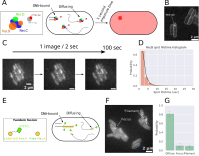
\includegraphics[width=.8\textwidth]{Figures/Fig1_endogenous.pdf}
    \caption{Imaging DSB repair in live \textit{E. coli}. \textbf{(A)} Scheme of our experimental protocol. The RecB subunit of the RecBCD complex is fused to a Halo-tag, bound by the JF549 fluorescent dye. A long exposure time (1 sec) makes diffusing molecules appear as diffuse signal in the cell, while DNA-bound molecules are visible as bright, diffraction-limited spots. \textbf{(B)} Example image of a RecB spot (white arrow). \textbf{(C)} Example images of a timelapse acquisition (1 image every 2 sec for 100 sec). \textbf{(D)} Histogram of the lifetime of RecB spots (bars) fitted with a mono-exponential decay function ($y=a.e^{-k.t}$) \textbf{(E)} Scheme of our RecA imaging system (from \cite{Wiktor2021}). Free and fluorescently labelled RecA are present in equal amounts in the cell. \textbf{(F)} Example image of RecA imaging under endogenous DNA damage. RecA is diffuse in most cells, a RecA focus and a RecA filament are visible in two of the cells (white arrows). \textbf{(G)} Proportions of cells containing the different RecA structures (dots: individual datasets, bars: average between datasets).}
    \label{Fig:endogenous}
\end{figure*}

To image Rec\-BCD in live \textit{E. coli}, we used a Halo-tag fusion to the RecB subunit, conjugated to the JF549 fluorescent dye (Figure \ref{Fig:endogenous}A). The fusion was previously used and characterised in the lab, ensuring specific one-to-one labelling of RecB molecules without adverse effects on the DNA repair process.\cite{Lepore2019a} To detect the binding of RecB to DNA, we applied the previously developed technique of localisation enhancement.\cite{Yu2006, Elf2007}  Since RecB is present at low copy numbers in \textit{E. coli} ($\sim$5 molecules per cell on average\cite{Lepore2019a}), imaging live cells with a long exposure time (1 second) made diffusing molecules appear as weak homogeneous signal in the cell, while DNA-bound molecules formed intense diffraction-limited spots (referred to throughout this article as RecB spots, Figures \ref{Fig:endogenous}B) The complete absence of similar spots in cells expressing the free Halo-tag from a plasmid confirmed that these structures were specific to RecB (Supp. Figure \ref{SIFig:freehalo_image}). Seeing RecB spots in cells that were not exposed to an exogenous source of DNA damage was unsurprising, as these cells are still subject to occasional endogenous DNA damage, such as replication fork collisions which were previously reported to affect $\sim$18\% of cells per cell cycle.\cite{Sinha2018}

Acquiring short timelapse videos (50 images over 100 seconds, Figure \ref{Fig:endogenous}C) allowed us to measure the lifetime of the RecB spots. The resulting histogram was well-fitted by a mono-exponential decay model ($y=a.e^{-k.t}$, with $a$ the fit amplitude and $k$ the dissociation rate from DNA), consistent with a single homogenous population of fluorescent spots (Figure \ref{Fig:endogenous}D). The fitted spot lifetime was 1.5 sec $\pm$ 0.1. This prolonged imaging of the RecB-Halo fusion was only possible thanks to the exceptional photostability of the JF549 dye, which displayed slow photobleaching and no blinking (Supp. Note \ref{note:dye_bleaching} and Supp. Fig. \ref{SIFig:dye_bleaching}).

%% RecA makes foci and filaments
\subsubsection*{RecA forms foci and filaments}
One of RecBCD's purposes when processing a DSB is to facilitate the loading of the RecA protein on single-stranded DNA. To broaden our view of the repair process downstream of RecBCD, we imaged a tandem fusion of RecA with the fluorescent protein SYFP2 (Figure \ref{Fig:endogenous}E).\cite{Wiktor2021} Based on the fluorescence distribution in the cells, we identified three states of RecA: diffuse, forming a bright focus, or forming an elongated filament (Figure \ref{Fig:endogenous}F). Because of the large diversity of shapes observed, especially for RecA filaments, the detection of RecA structures by rule-based algorithms was challenging. Therefore, we designed and trained a deep-learning algorithm capable of classifying individual cells based on the three types of structures cited above (see Methods and Supp. Figure \ref{SIFig:object_class}). This allowed us to quantify the fraction of cells where RecA is freely diffusing to 81\% $\pm$ 6, RecA foci to 10\% $\pm$ 4, and RecA filaments to 9\% $\pm$ 2 (Figure \ref{Fig:endogenous}G). This is consistent with a minority of cells experiencing DNA damage, and being engaged in the repair process.

% Part 2: Separating genuine RecB binding events
\subsection*{Finding DNA binding events}

\begin{figure*}[htbp]
    \centering
    \includegraphics[width=.8\textwidth]{Figures/Fig2_RecB_binding.pdf}
    \caption{RecB DNA binding under ciprofloxacin exposure. \textbf{(A)} Example kymographs of RecB throughout an acquisition. A short timelapse (100 sec) is acquired at a different position every 2 min for 75 min. \textbf{(B)} RecB spot lifetime histograms at 3, 10, 20 and 30 ng/mL ciprofloxacin (bars), fitted with a bi-exponential decay model (black line, fit components showed as dashed lines). \textbf{(C)} Probability of a spot corresponding to a DNA-bound RecB molecule, for cells over-expressing the Gam protein. Black dots show individual datasets, the black line is the average between them, and the red dashed line shows the smallest lifetime at which RecB spots have 95\% probability to be DNA-bound. \textbf{(D)} Recruitment rate of RecB on DNA at different ciprofloxacin concentrations. Black points show individual datasets, and bars the median value.}
    \label{Fig:lifetime_fits}
\end{figure*}

%% We add ciprofloxacin to increase the level of DNA damage
To gain more insight into DNA binding by RecB, we induced additional DSBs by adding the DSB-inducing antibiotic ciprofloxacin to agar pads before imaging. Cells were left to settle down on the pad for 10 min, after which 50-frame timelapse videos were acquired at a rate of one position every 2 min (Figure \ref{Fig:lifetime_fits}A) for 60 min. This allowed us to quantify RecB binding at different time points ranging from 15 to 75 min after the start of ciprofloxacin exposure.

%% RecB spot lifetime histograms change upon exposure to ciprofloxacin
%%% They are not well-fitted by a monoexponential decay (SI fig)
%%% We fit with a bi-exponential decay model
%%% Mention lifetimes/proportions, in table
Upon exposure to ciprofloxacin, the RecB spot lifetime histograms contained more long-lived spots. Fitting with a mono-exponential decay model as in Figure \ref{Fig:endogenous}D did not account well for these long-lived spots (Supp. Figure \ref{SIFig:monoexp_fits}), especially at the higher ciprofloxacin concentrations. This suggested that the new long-lived spots that appeared under exposure to ciprofloxacin corresponded to a new population of RecB spots, that had a slower dissociation rate from DNA than the ones observed under endogenous damage. Indeed, fitting with a bi-exponential decay model ($y = a_1.e^{-k_1.t} + a_2.e^{-k_2.t}$) accounted much better for the longer-lived RecB spots (Figure \ref{Fig:lifetime_fits}B). The bi-exponential fit outlined two populations of spots with different lifetimes: a short-lived one, with lifetimes ranging from 1.4 to 1.7 sec, and a longer-lived one, with lifetimes ranging from 10 to 14 sec (Table \ref{tab:fit_results}). Even though the short-lived spots always represented a majority of events (over 90\% of the spots), the proportion of long-lived spots tended to increase under higher ciprofloxacin exposure (from 1.4\% $\pm$ 0.3 under 3 ng/mL ciprofloxacin to 5.5\% $\pm$ 1.4 under 30 ng/mL ciprofloxacin).

\begin{table}[htbp]
    \centering
    \begin{tabular}{llll}
        \toprule
         &  & Lifetime (sec) & Population (\%) \\
        Ciprofloxacin & Type &  &  \\
        \midrule
        \multirow[t]{2}{*}{0} & Short & 1.4 $\pm$ 0.2 & 98.2 $\pm$ 1.0 \\
         & Long & 9.5 $\pm$ 9.7 & 1.8 $\pm$ 1.0 \\
        \cline{1-4}
        \multirow[t]{2}{*}{3 ng/mL} & Short & 1.5 $\pm$ 0.1 & 98.6 $\pm$ 0.3 \\
         & Long & 10.5 $\pm$ 1.3 & 1.4 $\pm$ 0.3 \\
        \cline{1-4}
        \multirow[t]{2}{*}{10 ng/mL} & Short & 1.7 $\pm$ 0.2 & 97.6 $\pm$ 0.6 \\
         & Long & 13.7 $\pm$ 2.3 & 2.4 $\pm$ 0.6 \\
        \cline{1-4}
        \multirow[t]{2}{*}{20 ng/mL} & Short & 1.6 $\pm$ 0.2 & 96.6 $\pm$ 0.8 \\
         & Long & 11.8 $\pm$ 2.1 & 3.4 $\pm$ 0.8 \\
        \cline{1-4}
        \multirow[t]{2}{*}{30 ng/mL} & Short & 1.7 $\pm$ 0.2 & 94.5 $\pm$ 1.4 \\
         & Long & 13.3 $\pm$ 2.2 & 5.5 $\pm$ 1.4 \\
        \cline{1-4}
        \bottomrule
        \end{tabular}
    \caption{Parameters derived from the spot lifetime histogram fits (Figures \ref{Fig:endogenous}D and \ref{Fig:lifetime_fits}B). The lifetime was calculated as the inverse of the fitted dissociation rate. Values are given as the median $\pm$ standard deviation over at least 3 independent datasets.}
    \label{tab:fit_results}
\end{table}

%% To check what these two populations are, we use the Gam protein to prevent DNA binding and fit with the same model
%%% Short-lived population stays, long-lived one is removed
%%% Interpretation: because of its size, the RecBCD-Halo-Gam complex can sometimes form spots (SI Note + SI Fig), which creates short spots
%%% Therefore, we are unable to assign short DNA binding events, but we can confidently detect longer DNA binding events
To determine whether both short- and long-lived spots resulted from RecB binding to DNA, we measured RecB spot lifetime in the presence and absence of ciprofloxacin while over-expressing the Gam protein of phage $\lambda$ from a plasmid. The Gam protein was previously shown to bind in place of DNA on the RecBCD complex\cite{Wilkinson2016}, and its overexpression is expected to abolish RecBCD binding to DNA. Accordingly, cells that over-expressed Gam and were exposed to high ciprofloxacin (30 ng/mL) showed little elongation compared to cells that did not overexpress Gam (Supp. Figure \ref{SIFig:Gam_cell_length}), indicating that most cells did not induce the SOS response, due to the inability of the RecBCD-Gam complex to bind to DSBs. The resulting RecB spot lifetime histograms showed a near-complete disappearance of the long-lived spots, while short-lived ones were still present (Supp. Figure \ref{SIFig:Gam_RecB_lifetimes_fits}). This was confirmed by fitting the histogram with our bi-exponential decay model, which found proportions of long-lived spots ($\sim$3\%) similar to those in wild-type cells that were not exposed to ciprofloxacin (2.6\%, Table \ref{tab:fit_results}). This confirmed that (i) long-lived RecB spots correspond to RecB molecules that have bound to DNA, and (ii) short-lived RecB spots can result from other causes than short-lived DNA binding (Supp. Note \ref{note:spurious_spots} and Supp. Figure \ref{SIFig:displacement_simul}). Spots that are visible only for a few seconds cannot be reliably assigned to one or the other category. However, based on the Gam overexpression data, we determined that any spot with a lifetime over 10 sec had 95\% probability to be DNA-bound (Figure \ref{Fig:lifetime_fits}C).

%% We use the number of spots and proportion of long-lived spots to estimate the rate of recruitment of RecB on the DNA (Fig 2D)
%% Mention/link to discussion on relationship between RecB recruitment rate and DSB formation rate
Whereas the lifetime of the fluorescent spots informs us on how long RecB stays bound to DNA, the rate of appearance of spots helps us estimate the rate of recruitment of RecB to DSBs under each DNA damage condition (Figure \ref{Fig:lifetime_fits}D). To achieve this, we quantified for each timelapse the total number of spots that belong to the "long-lived" (i.e. RecB bound to DNA) category. Since the short- and long-lived populations cannot be clearly separated from the lifetime histograms (Figure \ref{Fig:lifetime_fits}B), we used an "ensemble-level" approach. For each dataset, we multiplied the total number of spots that appeared during the timelapse by the proportion of long-lived spots retrieved from the lifetime histogram fits, which gave us an estimate of the number of DNA-bound RecB per timelapse, from which a number of recruitment events per hour can be calculated. We estimated that under endogenous damage or low ciprofloxacin concentrations, 1 to 2 RecB molecules are recruited to the DNA per hour on average. This is roughly consistent with the previous estimate of 18\% of cells generating an endogenous DSB per cell cycle\cite{Sinha2018} (see discussion). At ciprofloxacin concentrations above the MIC (30 ng/mL), the recruitment rate increased sharply to an average of 5 RecB recruited per hour. Furthermore, we expect that this recruitment rate gives a close estimate of the rate of formation of DSBs (see discussion).

% Part 3: Effects of DSBs and the repair process on the cell
\subsection*{Ciprofloxacin exposure induces formation of RecA filaments and nucleoid compaction}

\begin{figure*}[htbp]
    \centering
    \includegraphics[width=.8\textwidth]{Figures/Fig3_cell_response.pdf}
    \caption{Bacterial cell response to the induction of DSBs by ciprofloxacin. \textbf{(A)} Representative images of cells containing different RecA structures (diffuse fluorescence, foci or filaments) after 60 minutes of exposure to ciprofloxacin. Arrows point to representative examples of each of these structures. \textbf{(B)} Proportion of cells containing RecA foci or filaments. Black dots represent individual datasets, and bars the average between them. \textbf{(C)} Representative images of cells (segmented outline in grey) showing the nucleoid (green) and RecB-associated fluorescence (magenta). RecB spots (indicated by arrows) are located in close proximity to the nucleoid. \textbf{(D)} Overlay of nucleoid density (green area) and position of DNA-bound RecB molecules (magenta bars) along the cell's long axis, for different ciprofloxacin concentrations (0 to 30 ng/mL)}
    \label{Fig:reca_nucleoid}
\end{figure*}

%% We see a strong accumulation of RecA filaments (RecA foci seem to be transient and their number decreases over time)
To paint a more complete picture of the DNA repair process during ciprofloxacin exposure, we imaged the RecA protein fused to the fluorescent protein SYFP2. Figure \ref{Fig:reca_nucleoid}A shows the RecA-associated fluorescence in cells that have been exposed to different concentrations of ciprofloxacin for 60 minutes. In cells that were not exposed to ciprofloxacin, the RecA-associated fluorescence was mostly diffuse, and occasionally formed a bright focus. This is consistent with cells undergoing occasional endogenous DNA damage. As the ciprofloxacin concentration increases, RecA foci became more frequent, as well as filament structures.

To quantify more precisely the occurrence of foci and filaments at the different ciprofloxacin concentrations and durations of exposure, we used a custom-made deep-learning model to automatically classify cells depending on the presence of a focus, a filament, or neither of these structures (Figure \ref{Fig:reca_nucleoid}B, Supp. Figure \ref{SIFig:object_class}). The proportion of cells that contained RecA filaments was initially low under all ciprofloxacin concentrations ($<$20\%). After one hour of exposure the proportion of cells that contained a RecA filament had increased to $\sim$40\% at 20 ng/mL ciprofloxacin, and $\sim$60\% at 30 ng/mL. RecA foci on the other hand seemed to form quickly following ciprofloxacin exposure (present in $\sim$40\% of the cells after 15 min of exposure to 30 ng/mL ciprofloxacin) and come back to endogenous damage level after $\sim$1 hour. Taken together, these results show that RecA foci are transient structures in the repair process that do not accumulate under high DNA damage, whereas RecA filaments do accumulate, presumably when the homologous sequence cannot be found.

%% We imaged nucleoid and RecB in the same experiment
%% Ciprofloxacin exposure causes nucleoid compaction and centring
In \emph{E. coli}, the loading of RecA on DNA triggers the SOS response, which inhibits cell division, leading to cell filamentation. Previous studies have reported that the SOS response also triggers compaction of the bacterial nucleoid.\cite{Odsbu2014} To see if this was the case for breaks induced by ciprofloxacin in our experimental conditions, we stained DNA using the Sytox Green dye. The use of a green dye allowed us to concomittantly image RecB, and to correlate the position of DNA-bound RecB molecules with that of the nucleoid. Figure \ref{Fig:reca_nucleoid}C shows representative images of the nucleoid and DNA-bound RecB after 60 minutes of exposure to different concentrations of ciprofloxacin. In untreated cells, the nucleoid was often observed to be bi-lobed, which is consistent with cells growing exponentially, with high DNA replication activity. Upon exposure to ciprofloxacin, the cells appeared elongated, and the nucleoid was often compacted in the centre of the cell. As a result of the nucleoid compaction, the total fraction of the cell occupied by the nucleoid decreased, from 40\% on average in untreated cells to 31\% in cells exposed to 30 ng/mL of ciprofloxacin for an hour (Supp. Figure \ref{SIFig:nucleoid_compaction}). This compaction was accompanied by a centring of the nucleoid along the cell's long axis. Supp. Figure \ref{SIFig:nucleoid_position} shows that upon increasing exposure to ciprofloxacin (in time and concentration), the cells elongate, and nucleoids were increasingly centred.

%% Nucleoid and RecB position are correlated
%% Interpretation: RecB spot centring is due to nucleoid centring (not obvious: link to RecB recruitment rate, explain it happens after several rounds of DSBs)
As expected, DNA-bound RecB were found in close proximity to the nucleoid (Figure \ref{Fig:reca_nucleoid}C). Figure \ref{Fig:reca_nucleoid}D show the strong overlap between the spatial distribution of DNA-bound RecB spots and the nucleoid density in the cell (Supp. Figure \ref{SIFig:recb_nucleoid_timepoints} shows the same data after different durations of ciprofloxacin exposure). Due to nucleoid compaction and centring, both the nucleoid density and the position of DNA-bound RecB remained within $\sim$2 µm either side of the cell centre, despite the cells having elongated significantly.

%% Overall conclusion on RecA filaments, nucleoid compaction, and correlation of DNA-bound RecB position with nucleoid density
Upon exposure to ciprofloxacin, cells undergoing DSB repair load RecA at the break site, which we were able to detect as bright foci and filaments. At the lower (sub-MIC) ciprofloxacin concentrations, these structures were present in a low proportion of cells (10-20\%). At higher ciprofloxacin concentrations, RecA filaments were present in a large fraction of the cells (up to 40\%), hinting at an accumulation of long-lived RecA filaments unable to find a homologous sequence for repair. RecA loading on DNA also induces the SOS response. As a result, we observed compaction and centring of the bacterial nucleoid. DNA-bound RecB molecules were also found to be centred in elongated cells, consistently with DSBs forming on compacted nucleoids.

% Part 4: Mutants in the repair pathway
\subsection*{RecB dissociation does not depend on RecA loading}

\begin{figure*}[htbp]
    \centering
    \includegraphics[width=.75\textwidth]{Figures/Fig4_mutants.pdf}
    \caption{RecB binding to DNA in the \dreca\ and \teneighty\ mutant strains in the absence and presence of ciprofloxacin (30 ng/mL). \textbf{(A)} Representative brightfield images of wild-type (WT), \dreca\ and \teneighty\ mutants cells, in the presence and absence of ciprofloxacin (30 ng/mL). \textbf{(B)} Fitted lifetimes of RecB molecules on DNA. Black dots show individual datasets, and bars the median values. \textbf{(C)} Rate of recruitment of RecB to the DNA. Black dots show individual datasets, and bars the median values. \textbf{(D)} Representative overlay images of RecB-associated fluorescence (magenta) and the bacterial nucleoid (green). Segmented cell outline shown in grey. \textbf{(E)} Overlay of nucleoid density (green area) and position of DNA-bound RecB molecules (magenta bars) along the cell's long axis.}
    \label{Fig:mutants}
\end{figure*}

%% Effect of ciprofloxacin exposure on the different mutants
To better understand the factors that contribute to the dissociation of RecB from DNA, we imaged two different mutants (\dreca\ and \teneighty), in the presence and absence of 30 ng/mL ciprofloxacin. Figure \ref{Fig:mutants} shows brightfield images of cells that were not exposed to ciprofloxacin, and cells that were exposed to 30 ng/mL ciprofloxacin for 60 min. Supp. Figure \ref{SIFig:mutants_cell_lengths} shows the average cell length values across conditions and for the different ciprofloxacin exposure durations. As previously observed, wild-type cells show a clear response to exposure to 30 ng/mL ciprofloxacin, where the cell length increases significantly due to induction of the SOS response. In contrast to this, since the \dreca\ mutant is unable to form a RecA filament, it is also unable to induce the SOS response. Cell length therefore remains unchanged, even upon prolonged exposure to 30 ng/mL ciprofloxacin. The \teneighty\ mutant cells were slightly more elongated than wild-type cells in the absence of ciprofloxacin. This matches well with previous indications that this mutant has a higher baseline of SOS induction than wild-type cells in the absence of exogenous DNA damage.\cite{Lepore2023} Upon exposure to ciprofloxacin, the cell length of the \teneighty\ mutant increased, albeit slightly less on average than the wild-type's (Supp. Figure \ref{SIFig:mutants_cell_lengths}). This might be a reflection of \teneighty's inability to load RecA on the DNA, and the use of the alternative RecOR pathway leading to a weaker or delayed SOS response.

%% DNA binding lifetimes
As for the wild-type (WT) strain, we computed histograms of RecB spot lifetimes, and fitted them with a bi-exponential decay model (Supp. Figure \ref{SIFig:mutants_biexp_fits}), from which we extracted the slower rate, corresponding to the dissociation of DNA-bound RecB molecules. The corresponding lifetimes for DNA-bound RecB are shown on Figure \ref{Fig:mutants}B. In the \dreca\ mutant, the DNA-binding lifetime of RecB was similar to the wild-type ($\sim$10 sec). This suggests that RecA loading by RecBCD does not play a role in triggering the dissociation of RecBCD from DNA. Both in the presence and absence of ciprofloxacin, \teneighty\ stayed bound to DNA for longer than wild-type RecB ($\sim$20 sec). This could be due to the inability of \teneighty\ to digest the DNA it unwinds, making dissociation more challenging due to the DNA strands threading through the RecBCD complex.

%% RecB recruitment rate
Estimating the recruitment rate of RecB to the DNA provided additional insight into the dynamics of DSB processing in the \dreca\ and \teneighty\ mutants (Figure \ref{Fig:mutants}C). In the \dreca\ mutant, the rate of recruitment of RecB was increased compared to wild-type cells, both in the presence and absence of ciprofloxacin. As in both cases the rate of DSB formation is expected to be the same between the wild-type and the \dreca\ mutant, we can hypothesise that this higher rate of RecB recruitment to DNA is due to multiple recruitment events on the same original DSB. In the mutant cells, RecBCD processes the DNA, but the generated ssDNA cannot be coated with the RecA protein, and is therefore likely to be degraded by cellular endo- and exonucleases such as SbcCD. Degradation of the ssDNA would lead to a blunting of the DNA end, hence creating a new substrate for RecBCD binding. This deleterious cycle was previously reported to occur in cells lacking the RecA protein, eventually leading to full chromosome degradation\cite{Capaldo1975,Skarstad1993}. In our experiment, it results in multiple recruitments of RecB to DNA for each DSB.

%%% Intermediate recruitment in 1080 compared to WT and ΔrecA, probably resulting from a competition between ssDNA degradation + RecB reloading, and RecA loading + repair
In the \teneighty\ mutant, RecB recruitment is higher than in WT cells, but equivalent (in the absence of ciprofloxacin) or lower (in the presence of 30 ng/mL ciprofloxacin) to the level of RecB recruitment in the \dreca\ mutant (Figure \ref{Fig:mutants}C). Upon DSB recognition, \teneighty\ unwinds DNA without digesting it, and dissociates $\sim$2 times slower than wild-type RecB (Figure \ref{Fig:mutants}B). After RecBCD dissociation, we expect two competing pathways to take place. Either (i) the unwound ssDNA is digested by cellular endo- and exonucleases, creating a new RecBCD substrate; or (ii) RecOR displaces the SSB (Single-Strand DNA-Binding) protein and promotes RecA loading, allowing DNA repair by homologous recombination to proceed. As a result, RecB can be recruited on DNA several times for each DSB (similarly to the \dreca\ mutant), but the cycle of re-recruitment can be broken by the action of RecOR.

%% Compaction of the nucleoid
The differences in induction of the SOS response between the wild-type cells and the mutants resulted in different states of compaction for the bacterial nucleoid (Figure \ref{Fig:mutants}D, Supp. Figure \ref{SIFig:mutants_nucleoid_compaction}). Whereas in the wild-type, exposure to ciprofloxacin triggered compaction and centring of the nucleoid, the inability of the \dreca\ mutant to induce the SOS response resulted in two separate nucleoid regions at the cell poles. Furthermore, several cells appeared to have lower DNA content, consistent with RecBCD degrading large portions of the chromosome. Accordingly, the nucleoid occupied a smaller fraction of the cell in the \dreca\ mutant after exposure to ciprofloxacin (Supp. Figure \ref{SIFig:mutants_nucleoid_compaction}). In the RecB1080 mutant, the nucleoid appeared more disorganised than in wild-type cells, but still underwent compaction at the centre of the cell upon exposure to ciprofloxacin. Notably, the level of compaction of the nucleoid was slightly less important than in wild-type cells (38\% $\pm$ 9 of the cell occupied by the nucleoid after 75 min of exposure to ciprofloxacin, against 32\% $\pm$ 11 in the wild-type). This might again be a reflection of the less efficient RecA loading in this mutant, leading to delayed or weaker SOS response.

%% Colocalisation of RecB with the nucleoid
In all three strains, the localisation of DNA-bound RecB was consistent with that of the bacterial nucleoid, consistent with RecB being recruited to DSBs (Figures \ref{Fig:mutants}D and \ref{Fig:mutants}E). In the \dreca\ mutant, addition of 30 ng/mL ciprofloxacin did not change the spatial distribution of nucleoid density or DNA-bound RecB. This is consistent with \dreca\ cells being unable to induce the SOS response, and therefore not undergoing nucleoid compaction. In the \teneighty\ mutant, both nucleoid density and DNA-bound RecB distributions form a single peak at the cell centre, in the presence and absence of ciprofloxacin. This is consistent with the \teneighty\ mutant having a higher baseline of SOS induction than wild-type cells, as previously reported.\cite{Lepore2023} The slightly broader distribution of nucleoid density and DNA-bound RecB position in the \teneighty\ mutant exposed to ciprofloxacin compared to the wild-type is consistent with the lesser nucleoid compaction observed in this mutant (Figure \ref{SIFig:mutants_nucleoid_compaction}).

\begin{figure*}[htbp]
    \centering
    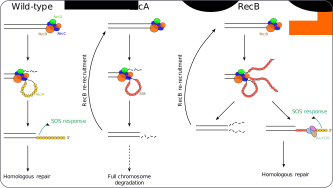
\includegraphics[width=\textwidth]{Figures/Fig_mutants_pathways.pdf}
    \caption{RecBCD recruitment pathways in wild-type \emph{E. coli}, \dreca\ and \teneighty\ mutants. \textbf{(Wild-type)} After DSB recognition, RecBCD degrades DNA until it recognises a Chi-site. It switches activity to create a 3' ssDNA overhang, and promotes RecA loading. The RecA-coated ssDNA can then be used for DNA repair by homologous recombination. \textbf{($\mathbf{\Delta}$reca)} In the absence of RecA, the 3' ssDNA is coated by SSB, and eventually digested by cellular nucleases. Blunting of the DNA end by digestion of the ssDNA creates a new substrate for binding of RecBCD. \textbf{(RecB$\mathbf{_{1080}}$)} Following DSB recognition, \teneighty\ unwinds DNA without digesting it. The unwound ssDNA can either be digested by nucleases, leading to a new blunt dsDNA end and RecBCD re-recruitment; or the RecOR complex displaces SSB to load RecA, allowing DNA repair by homologous recombination to proceed.}
    \label{Fig:pathways}
\end{figure*}

% Different pathways for RecB recruitment to DSBs in the different mutants
Our observations of cell elongation (Figure \ref{Fig:mutants}A), RecB recruitment to DNA (Figure \ref{Fig:mutants}C), and nucleoid position (Figure \ref{Fig:mutants}D) in the different mutant strains have led us to the model of RecB recruitment described in Figure \ref{Fig:pathways}. In wild-type cells, a DSB is recognised by RecBCD, which promotes RecA loading. The RecA filament triggers the SOS response, and is used for homology search and repair. In the \dreca\ mutant, the 3' ssDNA generated by RecBCD is first coated by SSB, and then degraded by cellular nucleases. This leads to blunting of the DNA end, creating a new substrate on which RecBCD can bind. This circle leads to multiple RecBCD recruitments per DSB, and eventually to full chromosome degradation. In the \teneighty\ mutant, RecBCD unwinds DNA without degrading it. After the ssDNA is coated with SSB, two competing pathways take place: either DNA degradation by nucleases leading to DNA-end blunting and re-recruitment of RecBCD, or displacement of SSB by RecOR and loading of RecA, leading to SOS induction and homologous repair.

\section*{Discussion}

% Accumulation of RecA filaments at high cipro might be due to extensive DNA damage and unsuccessful homology search
\subsection*{Accumulation of RecA filaments under high DNA damage}
Under exposure to high ciprofloxacin concentrations (20-30 ng/ml), we observed an accumulation of cells that contained a RecA filament (Supp. Figures \ref{SIFig:reca_structures}A and \ref{SIFig:reca_structures}B). At these ciprofloxacin concentrations, we have determined that cells undergo frequent DSBs, leading to multiple recruitments of RecB to DNA over the course of the experiment (up to 8 per hour, Figure \ref{Fig:recruitment}A). Given RecBCD's high processivity\cite{Wiktor2018}, such a high number of RecB recruitments would likely result in several kilobases of DNA being digested at different chromosomal locations. Furthermore, it has been previously reported that DSB repair by RecBCD takes ~15 min from RecBCD binding to a DSB to completion of the repair\cite{Wiktor2021}. At a rate of 8 RecB recruitments per hour, it is likely that several DSBs would be processed simultaneously, resulting in fragmentation of the bacterial chromosome. If a homologous copy of the break site is not present in the cell, we expect that the repair process will stall at the homology search stage, after formation of the RecA filament, which is consistent with our observation that a large proportion of cells contain RecA filaments following exposure to over-MIC ciprofloxacin concentrations.


\subsection*{Multiple RecB recruitments per DSB in the $\mathbf{\Delta}$\emph{reca} and RecB$\mathbf{_{1080}}$ mutants}

% Model of RecB recruitment to DNA
\begin{figure*}[htbp]
    \centering
    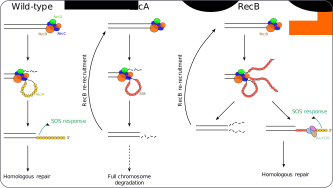
\includegraphics[width=\textwidth]{Figures/Fig_mutants_pathways.pdf}
    \caption{RecBCD recruitment pathways in wild-type \emph{E. coli}, \dreca\ and \geneteneighty\ mutants. \textbf{(Wild-type)} After DSB recognition, RecBCD degrades DNA until it recognises a Chi-site. It switches activity to create a 3' ssDNA overhang, and promotes RecA loading. The RecA-coated ssDNA can then be used for DNA repair by homologous recombination. \textbf{($\mathbf{\Delta}$reca)} In the absence of RecA, the 3' ssDNA is coated by SSB, and eventually digested by cellular nucleases. Blunting of the DNA end by digestion of the ssDNA creates a new substrate for binding of RecBCD. \textbf{(RecB$\mathbf{_{1080}}$)} Following DSB recognition, \teneighty\ unwinds DNA without digesting it. The unwound ssDNA can either be digested by nucleases, leading to a new blunt dsDNA end and RecBCD re-recruitment; or the RecFOR complex displaces SSB to load RecA, allowing DNA repair by homologous recombination to proceed.}
    \label{Fig:pathways}
\end{figure*}

Our observations of cell elongation (Supp. Figures \ref{SIFig:mutants_bf} and \ref{SIFig:mutants_cell_lengths}), RecB recruitment to DNA (Figure \ref{Fig:recruitment}), and nucleoid position (Figure \ref{Fig:nucleoid}) in the different mutant strains have led us to the model of RecB recruitment described in Figure \ref{Fig:pathways}. In wild-type cells, a DSB is recognised by RecBCD, which promotes RecA loading. The RecA filament triggers the SOS response, and is used for homology search and repair. In the \dreca\ mutant, the 3' ssDNA generated by RecBCD is first coated by SSB, and then degraded by the SbcCD and ExoI nucleases\cite{Zahradka2009}. This leads to blunting of the DNA end, creating a new substrate on which RecBCD can bind. This circle leads to multiple RecBCD recruitments per DSB, and eventually to full chromosome degradation. In the \geneteneighty\ mutant, RecBCD unwinds DNA without degrading it. After the ssDNA is coated with SSB, two competing pathways take place: either DNA degradation by SbcCD and ExoI leading to DNA-end blunting and re-recruitment of RecBCD, or displacement of SSB by RecFOR and loading of RecA, leading to SOS induction and homologous repair.

% Linking the RecB recruitment rate to DSB formation rate (ok in WT, more difficult in mutants due to re-recruitment to the same DSB)
\subsection*{Extrapolating the rate of DSB formation from the number of recruitments of RecB to DSBs}
Our experiments allowed us to estimate the number of recruitment of RecB to DSBs per hour, under different ciprofloxacin concentrations (Figure \ref{Fig:recruitment}A), and in the \dreca\ and \geneteneighty\ mutants (Figure \ref{Fig:recruitment}B). In the wild-type, the general pathway for DSB repair suggests that RecBCD is recruited once per DSB (Figure \ref{Fig:pathways}). We can therefore reasonably expect that the observed number of RecB recruitments observed matches with the number of DSBs formed (1 to 8 per hour, depending on ciprofloxacin concentration). In the \dreca\ and \geneteneighty\ mutants however, the disruptions to the DSB repair pathway lead to multiple RecB recruitments per DSB. We are therefore not able to estimate the rate of DSB formation in these mutants.

It should be noted that ciprofloxacin is expected to produce double-sided DSBs, hence leading to two RecB recruitments per break. We did not take this into account in our estimation of the DSB formation rate, as it has been previously suggested that the two sides of a DSB are kept in close proximity during DNA repair\cite{Vickridge2017,Keyamura2019}, and our imaging setup would not allow us to separate two RecB spots located close together. Indeed, our timelapse images of RecB binding seldom show two spots next to each other, further supporting the idea that we are not able to resolve RecBCD binding to both sides of a DSB.


\begin{funding}
    This work has been supported by Wellcome Trust Investigator Awards (Grant No. 205008/Z/16/Z awarded to M.E.K.), a BBSRC BB/S008012/1 responsive mode award (to M.E.K.), and a Marie Skłodowska-Curie Personal Fellowship (Grant No. 101063725-BARTAS) awarded to A.L.
\end{funding}

\begin{acknowledgements}
    We would like to thank Prof. David Leach for insightful discussions on DNA repair in \emph{E. coli}. We thank Mark Dillingham for sharing his knowledge on the biochemistry of RecBCD. We thank Johan Elf for kindly sharing the RecA-SYFP2 tandem fusion strain. We thank Jean Ollion for the development of BACMMAN and its associated tools, as well as the image analysis support he provided. We thank Elise Darmon for discussing results, and reviewing the manuscript.
\end{acknowledgements}

\begin{contributions}
    M.E.K. and D.T. conceived the experiments and designed the data analysis. D.T., A.L., and L.McL. built the strains. D.T. collected and analysed the data. M.E.K., D.T. and A.L. discussed the data. D.T. wrote the manuscript's first draft and created the figures. M.E.K., D.T. and A.L. revised the manuscript. L.McL., as the lab manager, oversaw order placements and maintained the lab organization. M.E.K. provided funding. All authors read, edited and approved the final manuscript.
\end{contributions}

\begin{interests}
    The authors declare no competing financial interests.
\end{interests}

\section*{Bibliography}
\bibliography{Bibliography}

\onecolumn
\newpage

%%%%%%%%%%%%%%%%%%%%%%%%%%%%%
% Supplementary Information %
%%%%%%%%%%%%%%%%%%%%%%%%%%%%%
\captionsetup*{format=largeformat}
\section{JF549 dye photobleaching kinetics}
\label{note:dye_bleaching} 

In our approach to estimating RecB binding times to DNA, the photostability of the fluorescent dye was of primary concern. Since we detect single molecules of RecB bound to DNA, two main photophysical behaviours were liable to cause artefacts in our data:
\begin{enumerate}
    \item Photobleaching (an irreversible loss of fluorescence) would limit the maximum number of frames we can track a DNA-bound RecB for, and would artefactually reduce the fitted binding times since some fluorescent spots might disappear due to photobleaching rather than unbinding from DNA
    \item Blinking (a transient loss of fluorescence) could cause repeated disappearance and reappearance of single molecules, and hence bias the computed binding times
\end{enumerate}

To address these concerns, we computed ensemble-level photobleaching curves by integrating the total fluorescence signal from the cells (Supp. Fig. \ref{SIFig:dye_bleaching}A). After 50 frames of laser exposure, a significant amount of photobleaching was noticeable (27\% $\pm$ 9 of the initial fluorescence remaining). The exact photobleaching rate of the dye in our experimental conditions can be estimated by fitting the photobleaching curve with an exponential decay function of the form $y=a.e^{-k.t}+b$ (with a the amplitude of the fit, k the bleaching rate, and b an offset to account for cellular auto-fluorescence). Since the bleaching rate is expected to mostly depend on experimental parameters that vary between but not within datasets (output laser power, HiLo angle), one bleaching rate was computed per dataset (Supp. Fig. \ref{SIFig:dye_bleaching}B). The true RecB dissociation rates were computed by subtracting the corresponding bleaching rates from the fitted spot disappearance rates.

All experimental photobleaching curves were well-fitted by a mono-exponential decay function. If significant blinking of the dye was occurring, we would expect photobleaching curves to follow more complex kinetics.\cite{} We therefore concluded that in our experimental conditions, the JF549 dye was not experiencing blinking, consistent with previous reports of the dye's outstanding photostability.\cite{}

%\clearpage

\section{Formation of RecB spots by the freely diffusing RecBCD-Halo-Gam complex}
\label{note:spurious_spots}
% Question: why are we seeing short-lived RecB spots when Gam prevents DNA binding?
In cells that overexpress the Gam protein, RecB is expected to be unable to bind DNA. Even though Gam overexpression prevents the apparition of long-lived RecB spots under exposure to ciprofloxacin, short-lived RecB spots remain present (Figure \ref{Fig:lifetime_fits}C). To understand how RecB spots can be formed in the absence of DNA binding, we simulated the expected displacements of a RecBCD-Halo-Gam complex according to the distribution of single displacements for a random 2D walk:
\begin{equation}
    P(r) = \dfrac{r}{2D_i t}e^{-\dfrac{r^2}{4D_i t}}
\end{equation}

with $D_i$ the apparent diffusion coefficient, and $t$ the frame time. Our previous work found a diffusion coefficient for RecB-Halo of $\sim$1.5 \ums. Assuming that the diffusion coefficient is proportional to the cube of the molecular weight, we expect a diffusion coefficient for the full RecBCD-Halo-Gam complex of $\sim$1 \ums. The frame time in our experiments is 1 second, but it is likely that a molecule that would stay immobile for a fraction of that time would still be visible as a spot. Although calculating a precise value is challenging, we used a ballpark estimate of 500 ms (half our frame time) of a molecule being immobile to be detected as a spot in our experiment. Supp. Figure \ref{SIFig:displacement_simul} shows the distribution of expected displacements under these parameters. Although most displacements would be too big to result in a bright fluorescent spot, a small fraction ($\sim$4\%) are smaller than 300 nm, and could create a spot. When factoring in the number of RecB molecules per cell (5 on average) and the number of frames in our timelapse (50), this would result in $\sim$10 RecB spots per cell, on the same order of magnitude as the number of spots observed in our experiments in the presence of the Gam protein (4.1 $\pm$ 0.2, mean $\pm$ sem).

\clearpage

\setlength\intextsep{40pt}

%% SUPPLEMENTARY FIGURES

% Strains table
\begin{supptable}[htbp]
    \centering
    \begin{tabular}{lll}
        \toprule
        Name & Description & Reference\\
        \midrule
        MEK2623 & MG1655 \textit{recB::halotag recA::syfp2} & this work\\
        MEK2622 & MG1655 \textit{recB::halotag $\Delta$recA} & this work \\ % = AL133_1
        MEK2324 & MG1655 \textit{recB1080::halotag HK022::psfiA-GFP} &  \\ % Alessia's article
        MEK65 & MG1655 \textit{recB::halotag} & \cite{Lepore2019a} \\
        BHC9 & MG1655 \textit{$\Delta$recA} & Ref? \\
        \bottomrule
    \end{tabular}
    \caption{List of bacterial strains used in this study}
    \label{SItab:strains}
\end{supptable}

% Plasmids table
\begin{supptable}[htbp]
    \centering
    \begin{tabular}{lll}
        \toprule
        Name & Description & Reference\\
        \midrule
        pSF1 & Expression of HaloTag under the control of the pBAD promoter & \cite{Lepore2019a} \\
        pDT6 & GamL inserted into pBAD322K by restriction cloning & \cite{Wilkinson2016} \\
        \bottomrule
    \end{tabular}
    \caption{List of bacterial plasmids used in this study}
    \label{SItab:plasmids}
\end{supptable}

% Data analysis pipeline
\begin{suppfigure*}[htbp]
\begin{center}
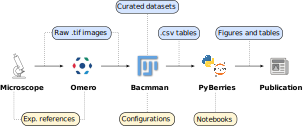
\includegraphics[width=\textwidth]{SI_Figures/Data_analysis_workflow.pdf}
\end{center}
\caption{Data storage and analysis pipeline used in this study. Blue labels indicate stored data and yellow labels indicate code and references that would allow reproducing the different analysis steps.}
\label{SIFig:analysis_workflow}
\end{suppfigure*}

%\clearpage

% Object classification workflow
\begin{suppfigure*}[htbp]
    \begin{center}
    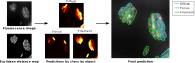
\includegraphics[width=\textwidth]{SI_Figures/ObjectClassifier.pdf}
    \end{center}
    \caption{Classification of cells according to the RecA structures they contain by our in-house Unet-based deep-learning network.}
    \label{SIFig:object_class}
\end{suppfigure*}

% Example image of freely diffusing halo-tag + JF549
\begin{suppfigure*}[htbp]
\begin{center}
\includegraphics[width=.5\linewidth]{SI_Figures/Free_Halo_image.png}
\end{center}
\caption{Fluorescence image of freely diffusing Halo-tag expressed from a pBAD plasmid in MG1655 \textit{E. coli} cells.}
\label{SIFig:freehalo_image}
\end{suppfigure*}

% Monoexponential fit of WT data, all cipro concentrations
\begin{suppfigure*}[htbp]
\begin{center}
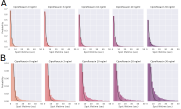
\includegraphics[width=\linewidth]{SI_Figures/Monoexp_fits_cipro.pdf}
\end{center}
\caption{Histograms of RecB spot lifetime (bars) under exposure to ciprofloxacin, with overlaid mono-exponential decay fits ($y=a.e^{-k.t}$, black line).}
\label{SIFig:monoexp_fits}
\end{suppfigure*}

%\clearpage

% Cell length under Gam over-expression, 0 and 30 ng/mL cipro
\begin{suppfigure*}[htbp]
    \begin{center}
    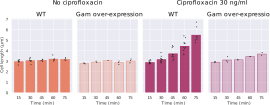
\includegraphics[width=\linewidth]{SI_Figures/Cell_length_Gam.pdf}
    \end{center}
    \caption{Length of cells that over-express Gam or not (WT), under exposure to 0 or 30 ng/mL ciprofloxacin. Black dots show indvidual datasets, and bars the average between them.}
    \label{SIFig:Gam_cell_length}
\end{suppfigure*}

% Bi-exponential fit of RecB spot lifetimes under Gam over-expression, 0 and 30 ng/mL cipro
\begin{suppfigure*}[htbp]
    \begin{center}
    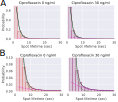
\includegraphics[width=\linewidth]{SI_Figures/Gam_lifetimes_fits.pdf}
    \end{center}
    \caption{Histograms of RecB spot lifetime (bars) in cells over-expressing the Gam protein with overlaid bi-exponential decay fits ($y=a_1.e^{-k_1.t} + a_2.e^{-k_2.t}$, black line) and individual fit components (dashed lines).}
    \label{SIFig:Gam_RecB_lifetimes_fits}
\end{suppfigure*}

% Photobleaching figure (curves + fitted rates)
\begin{suppfigure*}[htbp]
\begin{center}
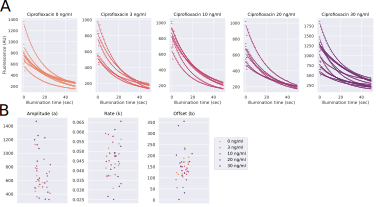
\includegraphics[width=\textwidth]{SI_Figures/SIFig_bleaching.pdf}
\end{center}
\caption{Ensemble-level photobleaching of the JF549 dye. (A) Average background-subtracted fluorescence for 5 independent datasets (solid lines), overlaid with the photobleaching rate fit ($y=a.e^{-k.t}+b$, dotted line). (B) Fitted model parameters for each of the 5 datasets: amplitude (a), offset (b) and photobleaching rate (k).}
\label{SIFig:dye_bleaching}
\end{suppfigure*}

% Displacements simulation
\begin{suppfigure*}[htbp]
    \begin{center}
    \includegraphics[width=.8\textwidth]{SI_Figures/Displacements_distribution.pdf}
    \end{center}
    \caption{Histogram of expected displacements for a molecule diffusing at 1 \ums\ over a 500 ms frame time.}
    \label{SIFig:displacement_simul}
\end{suppfigure*}

% Mutants: RecB spot lifetime histogram bi-exp fits
\begin{suppfigure*}[htbp]
    \begin{center}
    \includegraphics[width=.8\textwidth]{SI_Figures/Mutants_RecB_fits.pdf}
    \end{center}
    \caption{RecB spot lifetime histograms for wild-type (WT), \dreca, \teneighty\ and \teneighty -\dreca\ strains, at 0 and 30 ng/mL ciprofloxacin, fitted with a bi-exponential decay model (black line, fit components showed as dashed lines).}
    \label{SIFig:mutants_biexp_fits}
\end{suppfigure*}


\end{document}
